%!TEX root = ../Fast_Contour_Tracing_Algorithm.tex
% -*- root: ../Fast_Contour_Tracing_Algorithm.tex -*-

\section{Experimental Result}

For comparing the proposed algorithm with conventional algorithms, we perform experiment for determining their accuracy, speed, and stored data size. Table \ref{table:exp_environment} shows the experimental environment.

\begin{table}[h]
	\centering
	\begin{tabularx}{0.9\textwidth}{YYY}
		\hline
		  &  Desktop & Notebook(Samsung Sens V20) \\ 
		\hline
		CPU & Intel Core 2 CPU 6300 1.86 GHz & Intel Pentium 4 1.80GHz \\
		Memory & 512 MB & 256 MB \\  
		HDD & Samsung UDMA 133 7,200RPM 8MB Buffer & Hitachi UDMA 100 4,200RPM 2MB Buffer \\
		O/S & \multicolumn{2}{c}{Microsoft Windows 7} \\
		Development & \multicolumn{2}{c}{Microsoft Visual Studio 2013} \\ 
		\hline
	\end{tabularx}
	\caption{Experimental Environment}
	\label{table:exp_environment}
\end{table}	

We experimented on nine CCITT standard fax images with 200 DPI (dots per inch) \textcolor{red}{[14]}. All these images have $1,728 \times 2,339$ pixels and a file size of 11,842 KB. Table \ref{table:ccitt} shows the document type of these images and the total number of contour pixels. We used these large sized images because they a number of various types of contours, and they are useful to compare the efficiencies with regard to parameters such as processing time and accuracy of the trace results of the contour tracing algorithms.

\begin{table}[h]
	\centering
	\begin{tabularx}{0.7\textwidth}{YYY}
		\hline
		Index & Type & Total number of contour pixels \\
		\hline
		1 & Business letter & 81,189 \\
		2 & Circuit diagram & 50,825 \\
		3 & Sales order table & 152,489 \\
		4 & French document & 312,812 \\
		5 & Technical paper & 157,377 \\
		6 & Technical graph & 98,579 \\
		7 & Japanese document & 283,717 \\
		8 & Handwritten memo & 97,031 \\
		9 & Facsimile test chart & 453,721 \\
		\hline
	\end{tabularx}
	\caption{CCITT Fax Standard Images}
	\label{table:ccitt}
\end{table}	

In order to compare the proposed algorithm with conventional algorithms, we used the experimental method described in \cite{Danielsson1981Improvement} for determining the start pixels of the outer and inner contours of the images. In other words, whenever any untraced contour pixel is searched using a raster scan from the left-top to the right-bottom of the images, this pixel is regarded as the start pixel and the tracer starts contour tracing. If the contour is an outer contour, the tracer's initial direction is assigned as East (``E''). On the contrary, in the case of the inner contour of an object e.g., ``e,'' ``p,'' ``q,'' ``R,'' and ``o,'' the tracer's initial direction is assigned as West (``W''), as shown in figure \textcolor{red}{2 (a)}.

In the experiments, we did not consider the TPA, since the initial condition of the TPA\cite{Ghuneim2015Contour,Pavlidis2012Algorithms} is that it must start with white left (``L''), left-rear (``W''), and right-rear (``R'') pixels, which is not satisfied in some of the inner contours. Figure \textcolor{red}{15} shows an example of this violation. In our experimental situation, there were many cases in which such conditions were not satisfied; therefore, we could not perform identical experiments and meaningful data was not obtained for comparing the trace results with those of the other methods. 

\subsection{Accuracy}

The accuracy of contour tracing involves determining how accurately the tracing algorithm traces, and we measure it by counting the number of pixels traced. Firstly, we apply each algorithm to the test images and mark the tracing on the images. Then we count all the marked contour pixels in the images. Therefore, even if a pixel is traced several times, it is counted only once. Table \JHMEMO{7} shows the results of the comparison between the proposed algorithm and the conventional ones. In the table, \JHMEMO{``total number''} implies the total number of contour pixels, including the inner corner, outer corner, inner-outer corner, and straight line pixels. In this result, the MNT and RSA traced the least number of pixels as contours because they could not trace the inner corner pixels. the SBF has inconsistencies with regard to the inner-outer corner and inner corner types; therefore, it traced lesser number of pixels as compared to the ISBF and proposed algorithm.  Further, the MSBF has inner corner inconsistencies that are similar to those of the SBF; the MSBF traced lesser number of pixels as compared to the proposed algorithm and ISBF. The proposed algorithm shows that $99.5\%$ of the total contour pixels were found to be the same as those in the case of the ISBF and it has the maximum total number of traced contour pixels. In conclusion, the proposed algorithm produced the best results with regard to tracing accuracy.
Figure 16 shows the traced images resulting from the MSBF and proposed algorithm. In this figure, (a) could not trace some of the inner corner pixels but (b) traced all the corner pixel types without any inconsistency. Moreover, as the proposed algorithm can classify each corner type, it can trace the selected type of contour pixels by omitting some cases, as shown in figure 9 (b). For example, if we remove the tracing cases (1) and (6) from the other cases, we can obtain a result without inner corner tracing, and it is the same as the result of the MNT and RSA. Figure \textcolor{red}{17 (b)} shows an image that is traced using the proposed algorithm without inner corners, and it shows that the image is consistently traced without inner corners.

\subsection{Speed}

In order to measure the tracing time for each algorithm, we performed each algorithm 10 times per image and calculated the average time. We used the GetTickCount() function supported by Microsoft Visual C++ 6.0 to measure the processing time. Tables \textcolor{red}{8 and 9} show the average processing time of each algorithm used for tracing the images, and a linear model for estimating the process time as the number of traced pixels increases by using the least-square estimation (LSE) method. In the tables, the average processing time per traced contour pixel is obtained by dividing the total processing time by the total number of traced contour pixels. They are measured on the desktop and notebook separately.

Moreover, figure \textcolor{red}{18} illustrates a graph that uses data from tables \textcolor{red}{7 to 9}. As shown in figures \textcolor{red}{18 (a) and (b)}, the proposed algorithm had the best performance in the case of the desktop, i.e., it had the least average processing time and showed the least increase in the ratio of process time to number of traced contour pixels, as shown in the LSE. In particular, although the proposed algorithm traced most of the numerous contour pixels in each image, it has the best or good performance when compared with the conventional algorithms. On the contrary, the SBF had the least average processing time for images and the least ratio from the LSE in the case of the notebook, and the proposed algorithm is second in rank based on the average processing time and LSE. from these experimental results the SBF is not the best algorithm for the note book because the ratio of the number of traced contour pixels is only approximately $92\%$ of the proposed algorithm. Due to this reason, the proposed algorithm has better performance than the other algorithms for the number of traced contour pixels and the processing time.

\subsection{Memeory consumption}

The proposed algorithm does not save all the contour pixels, but it saves only the representative points and the inner-outer corner pixels. Table \textcolor{red}{10} shows the data size acquired from the above experiments on CCITT standard fax images. It shows the data sizes of traced contour pixels and its compressed data. The number of traced contour pixels $(A)$, which are same results from table \textcolor{red}{7} and the $C$ and $D$ in the table are numbers of the representative points and the inner-outer corner points of the traced contour pixels. $A$ and $C$ are the number of $(x, y)$ coordinates, and $D$ represents the number of inner-outer corners that comprise $(x, y)$ coordinates and the type of inner-outer corner. The benefit of storing only the representative points based on the vertex of the contour pixel is that it can dramatically reduce the data size. This experimental results showed that the proposed algorithm reduced the data size to {19~60\%} of the memory used when all the contour pixels were stored, as shown in Table \textcolor{red}{10}.

\subsection{Restoration}

Figure \ref{fig:image19} shows an example of retrieval points and a restoration result obtained by using the proposed restoration algorithm. Figure \ref{fig:img19-a} is an example image that has all the contour pixel types, and it depicts the representative points and inner-outer corner points for contour description and restoration. This image has two contours, namely, an outer contour and an inner contour that includes two inner-outer corners. Table \textcolor{red}{11} describes these data and figure \textcolor{red}{18 (b)} shows the restoration results, which are retrieved using the data from table \textcolor{red}{11}. In the figure, the restored contour accurately represents the original contour pixels.

%%% Image 19
\begin{figure}[htbp]
	\centering
	\subfloat[]{ 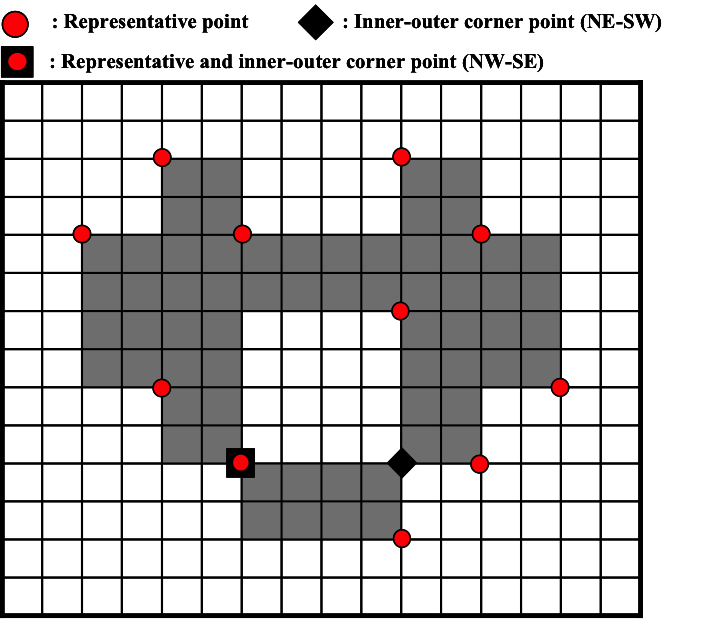
\includegraphics[width=7cm, height=6cm]{5.ExperimentalResult/fig19_a.png} \label{fig:img19-a} }
	\subfloat[]{ 
\includegraphics[width=7cm, height=5.25cm]{5.ExperimentalResult/fig19_b.png} \label{fig:img19-b} }
	 
	\caption{Example of restoration of contour pixels. \protect\subref{fig:img19-a} Original image and its saved points for restoration \protect\subref{fig:img19-b} Restoration by saved data}
	\label{fig:image19}
\end{figure}

Figure \ref{fig:image20} shows the result for the CCITT \#1 image using the proposed restoration algorithm. Figure \ref{fig:img20-a} represents the result of contour tracing and \ref{fig:img20-b} depicts the result of restoration from the compressed contour data. To verify the identity, we compared the contour pixels of the two images and they are identical with regard to the number of contour pixels and the pixel coordinates, i.e., the contour pixels in the restoration result is the same as the original contour pixels. As shown in figures \ref{fig:image20} \textcolor{red}{figures 19 and 20}, these experiments proved that the proposed algorithm could trace the inner and outer contours, and it could store the results using lesser memory by storing only the representative points and inner-outer corner points instead of all the contour pixels; moreover, it could accurately restore all the contour pixels correctly from the compressed data. Besides, as shown in \cite{Miyatake1997Contour}, compressed data based on vertex contours guarantee precise enlarging.

%%% Image 20
\begin{figure}[htbp]
	\centering
	\subfloat[]{ 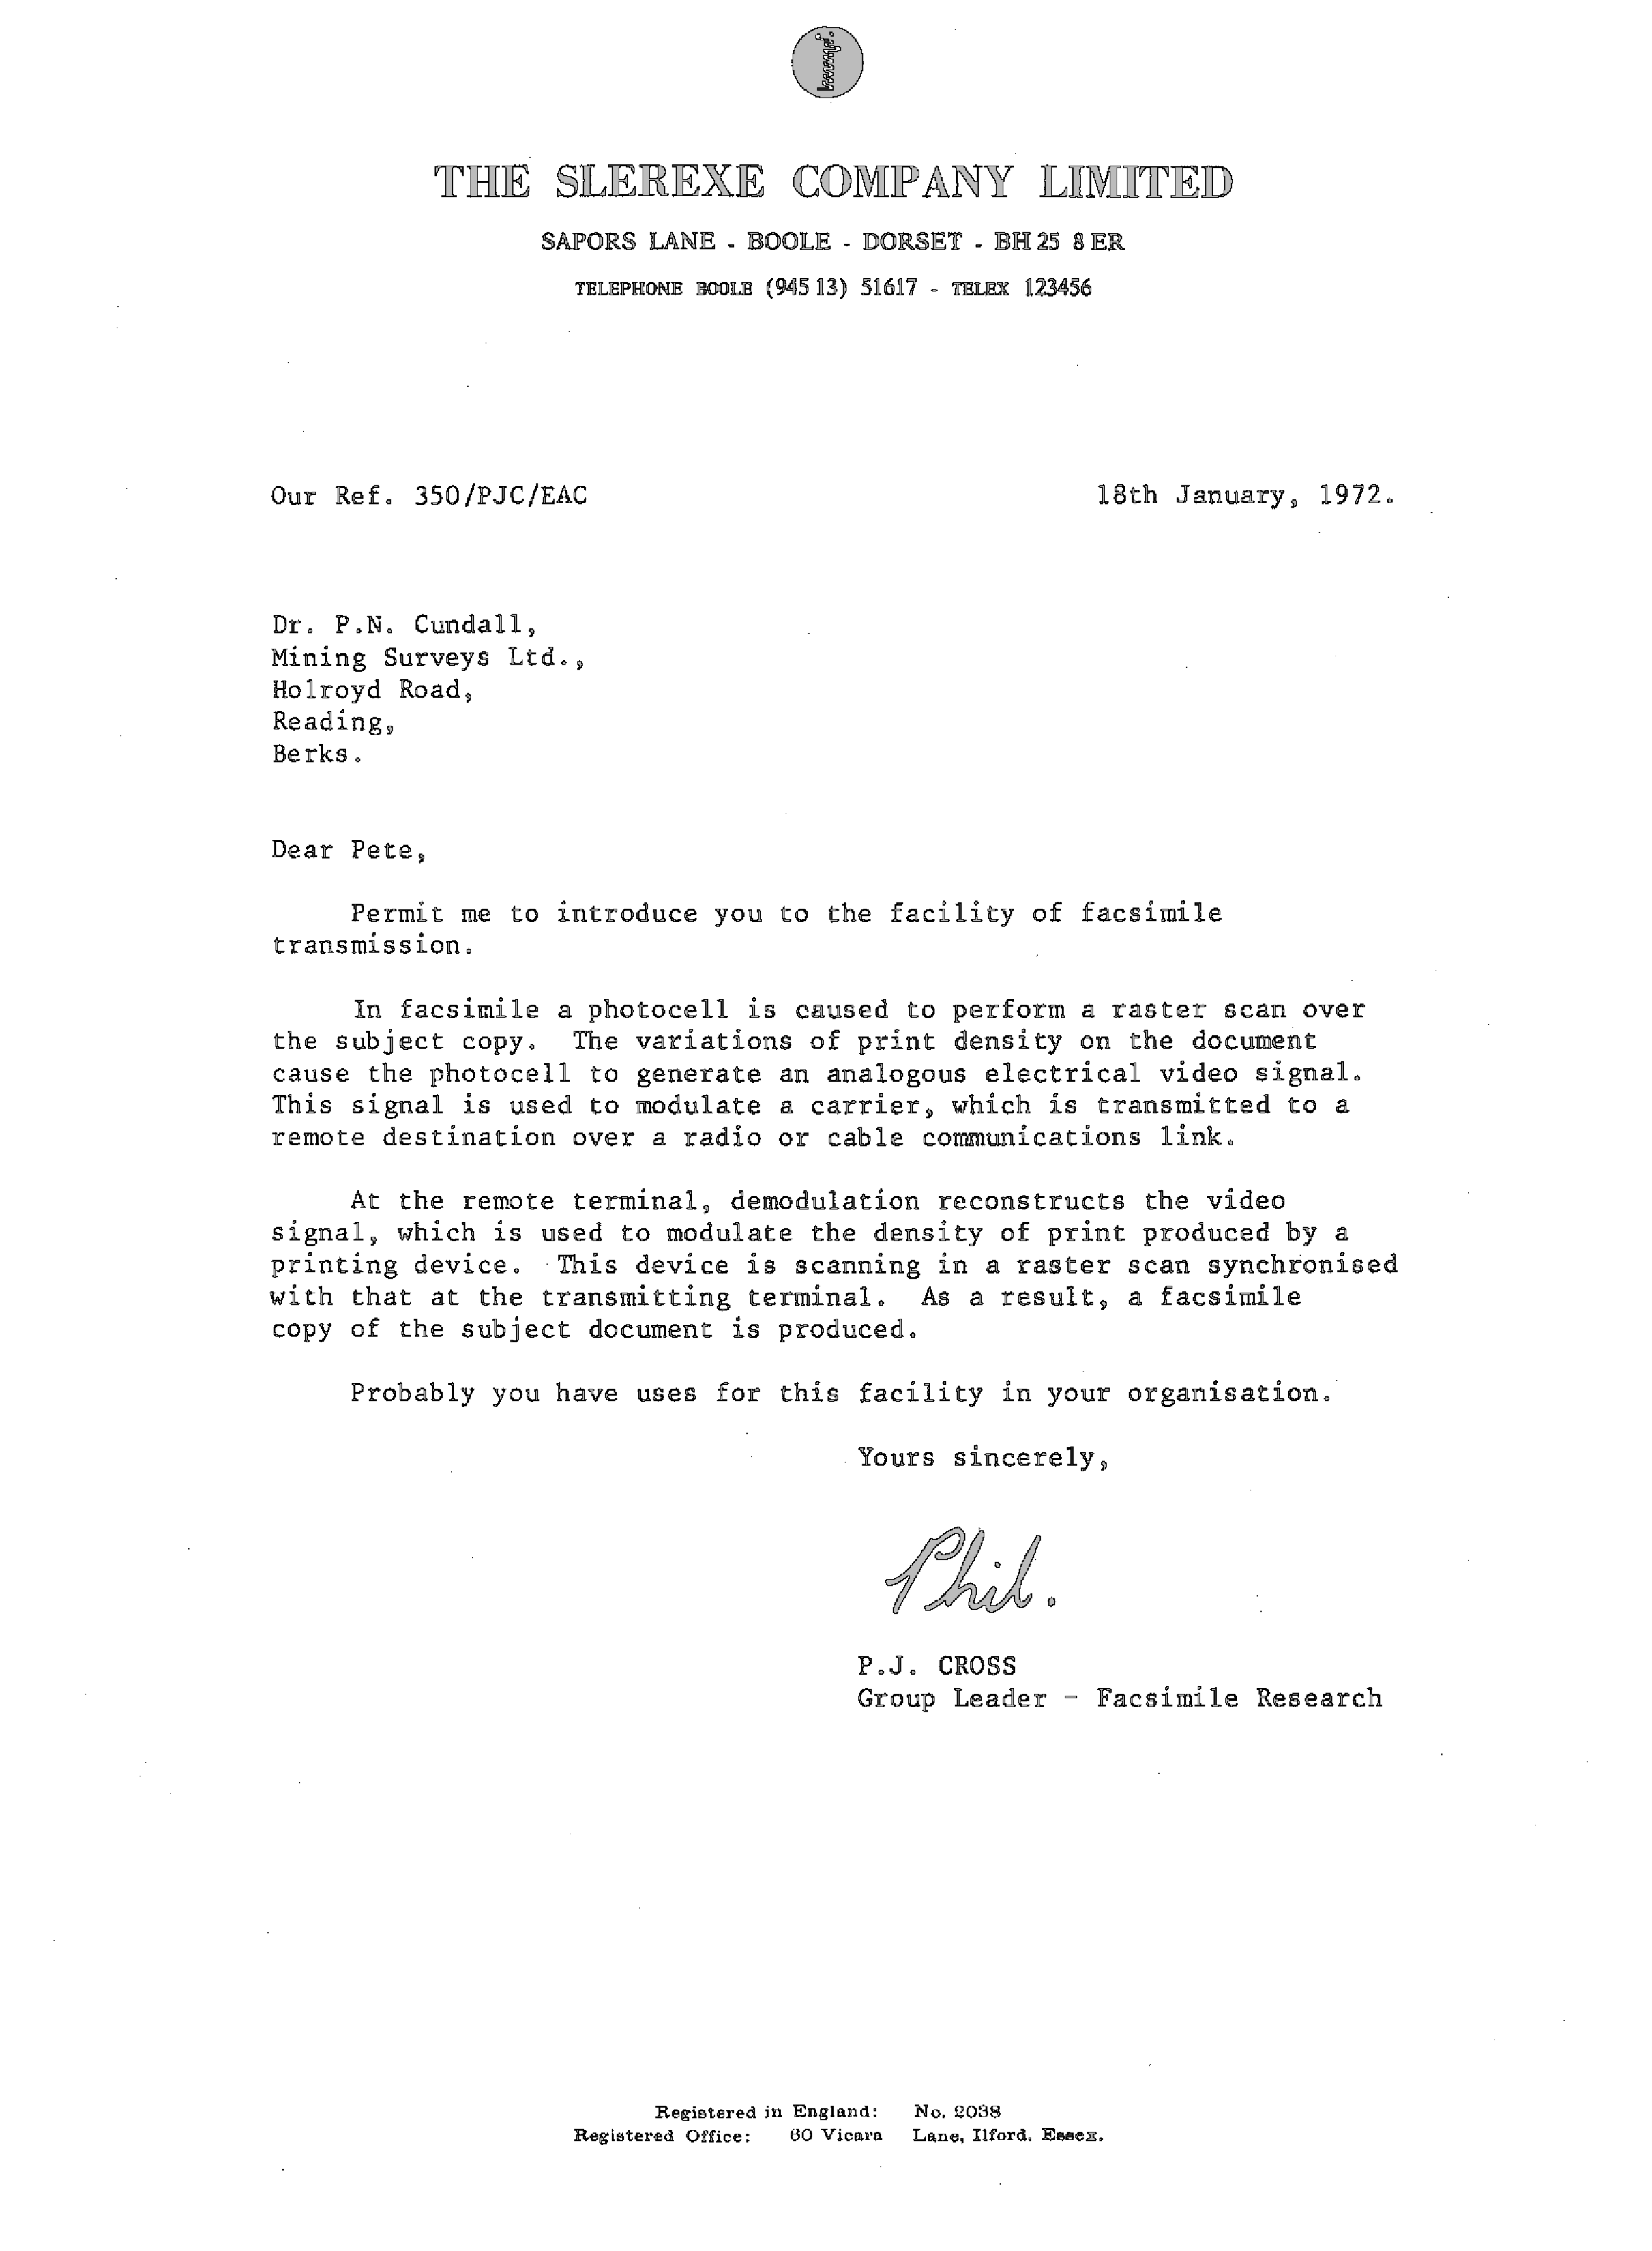
\includegraphics[width=0.5\textwidth]{5.ExperimentalResult/fig20_a.png} \label{fig:img20-a} }
	\subfloat[]{ 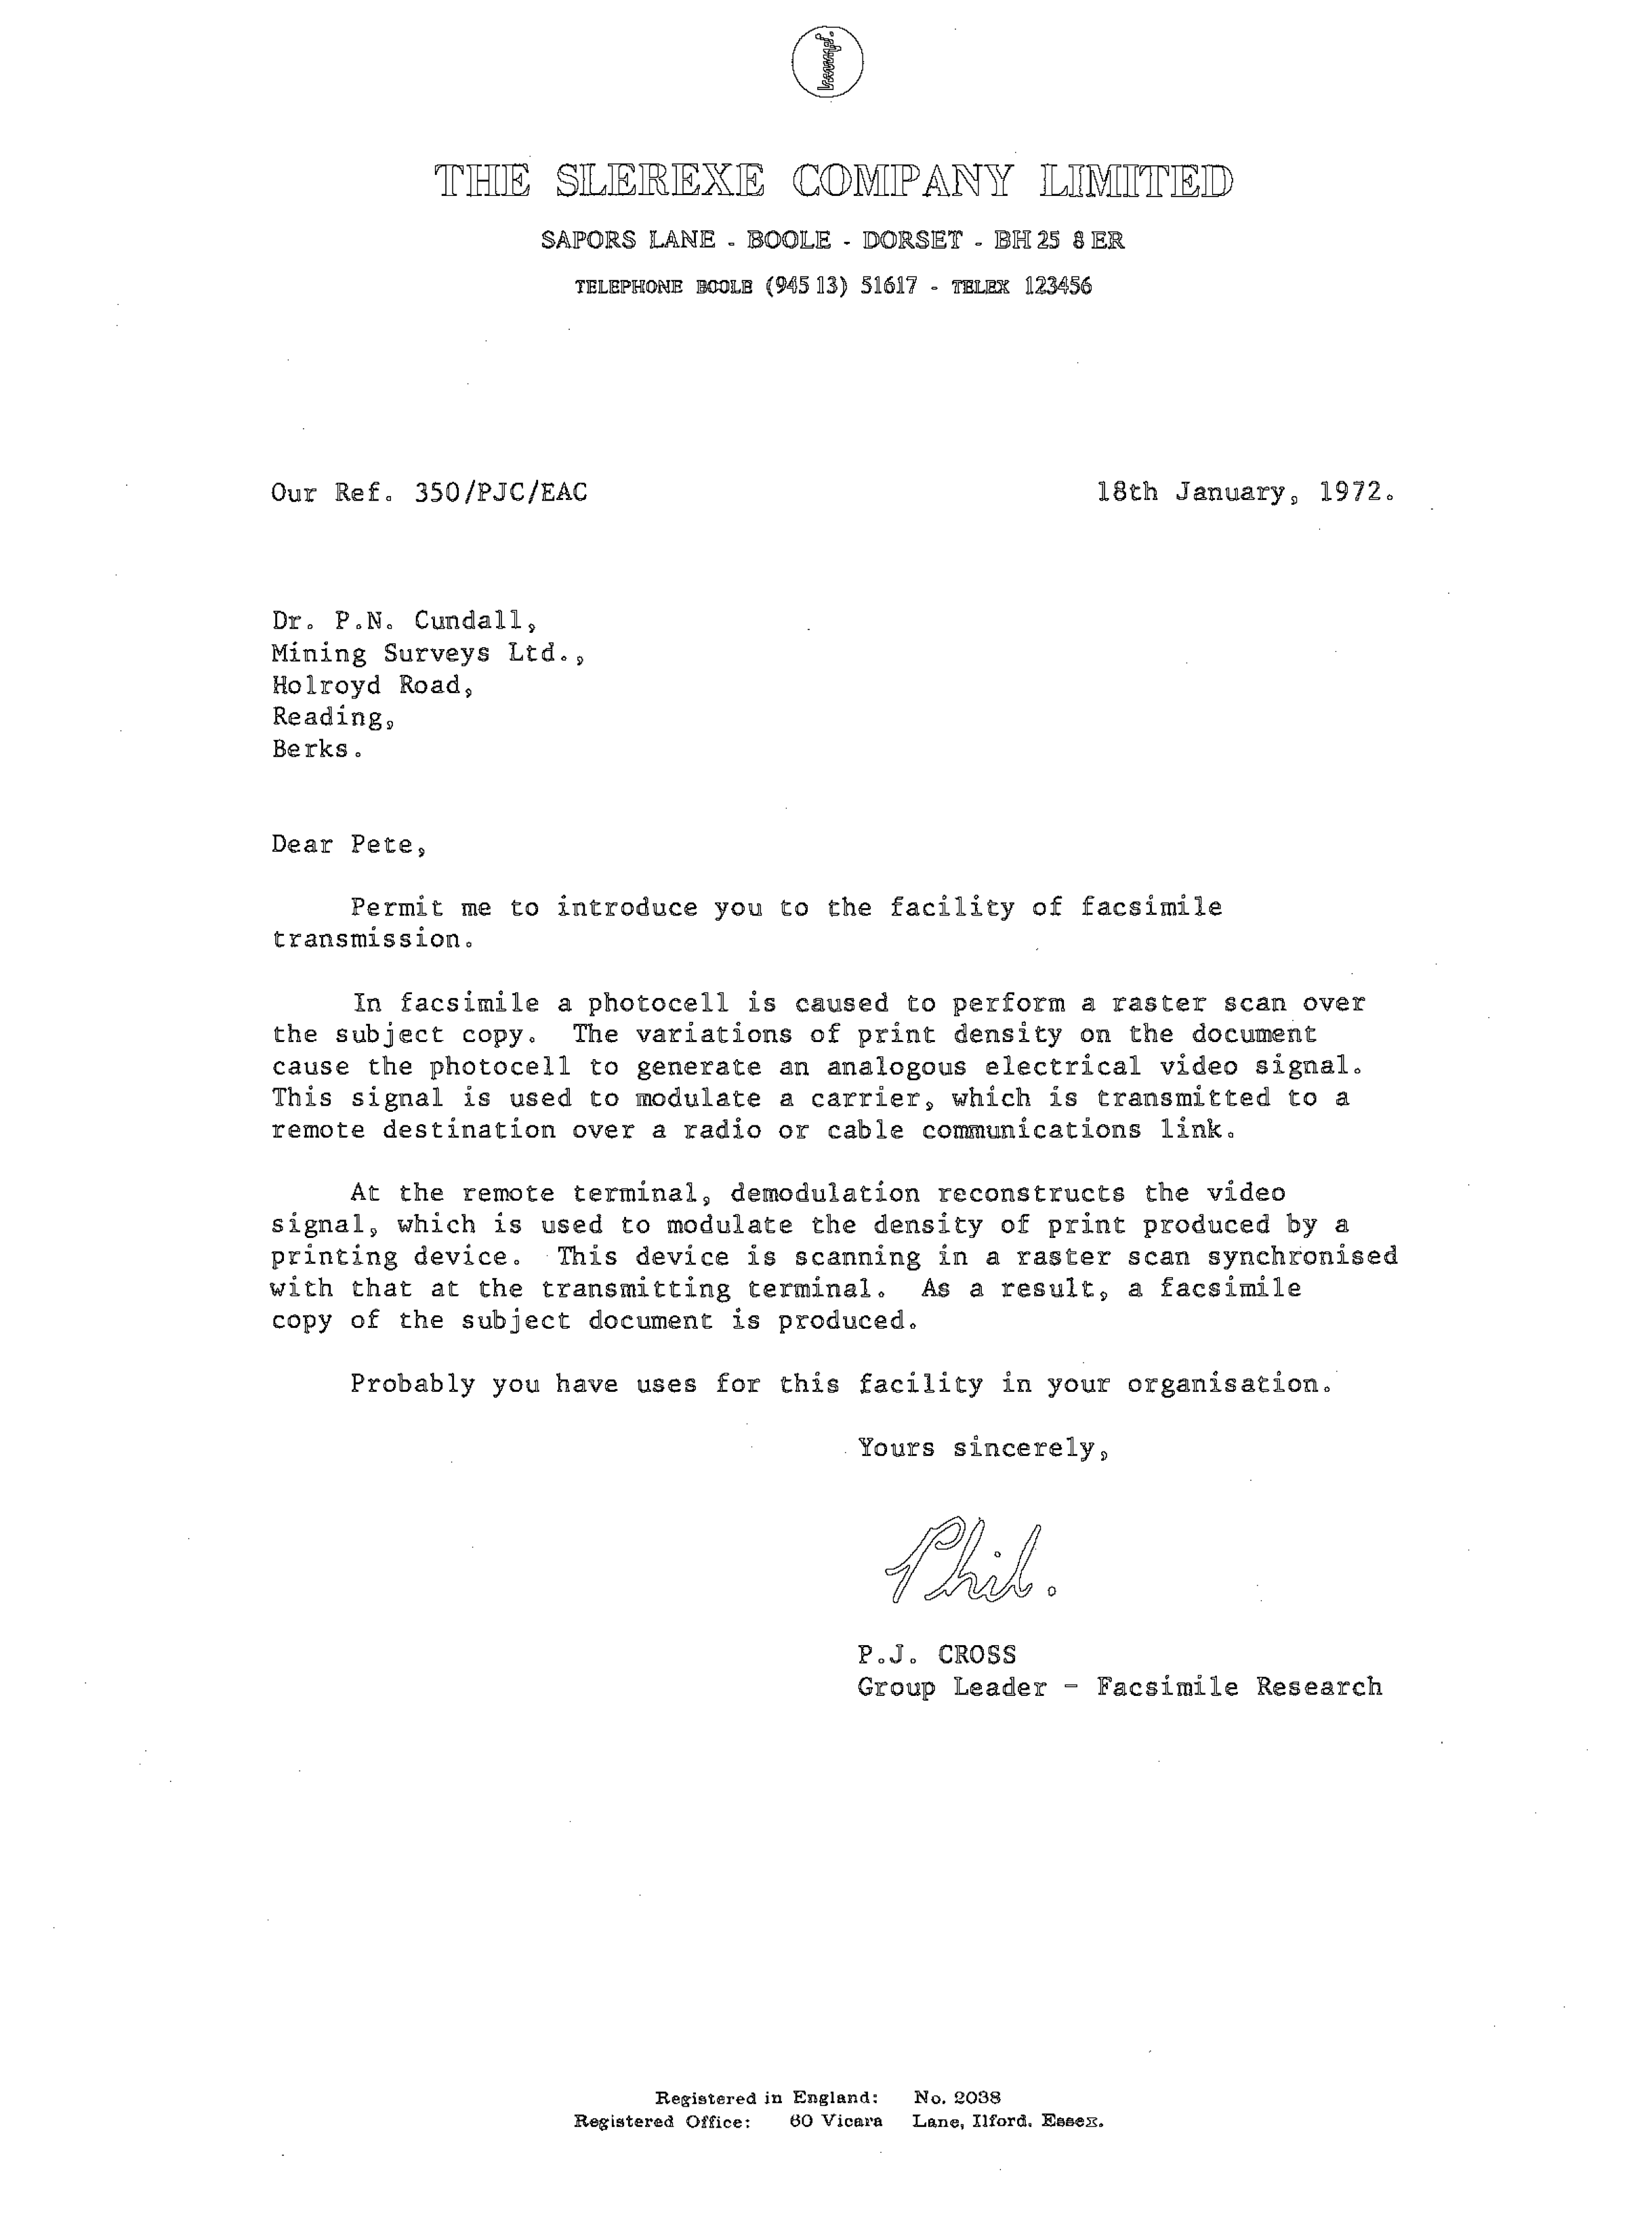
\includegraphics[width=0.5\textwidth]{5.ExperimentalResult/fig20_b.png} \label{fig:img20-b} }
	 
	\caption{Result of experiment for CCITT \#1. Red pixels are contour pixels. \protect\subref{fig:img20-a} Result of contour tracing \protect\subref{fig:img20-b} Result of contour restoration}
	\label{fig:image20}
\end{figure}

\subsection{Limitations}

%%% Image 21
\begin{figure}[htbp]
	\centering
	\subfloat[]{ 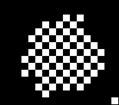
\includegraphics[width=4.5cm, height=4.5cm]{5.ExperimentalResult/fig21-a.png} \label{fig:img21-a} }
	\subfloat[]{ 
\includegraphics[width=4.5cm, height=4.5cm]{5.ExperimentalResult/fig21-b.png} \label{fig:img21-b} }
	\subfloat[]{ 
\includegraphics[width=4.5cm, height=4.5cm]{5.ExperimentalResult/fig21-c.png} \label{fig:img21-c} }
	 
	\caption{Example of untraced contour pixels caused by missing starting pixel CCITT Image \#9 from (1093, 1766) to (1108, 1780). \protect\subref{fig:img21-a} Original image \protect\subref{fig:img21-b} Traced by ISBF \protect\subref{fig:img21-c} Traced by the proposed algorithm}
	\label{fig:image21}
\end{figure}

%%% Image 22
\begin{figure}[htbp]
	\centering
	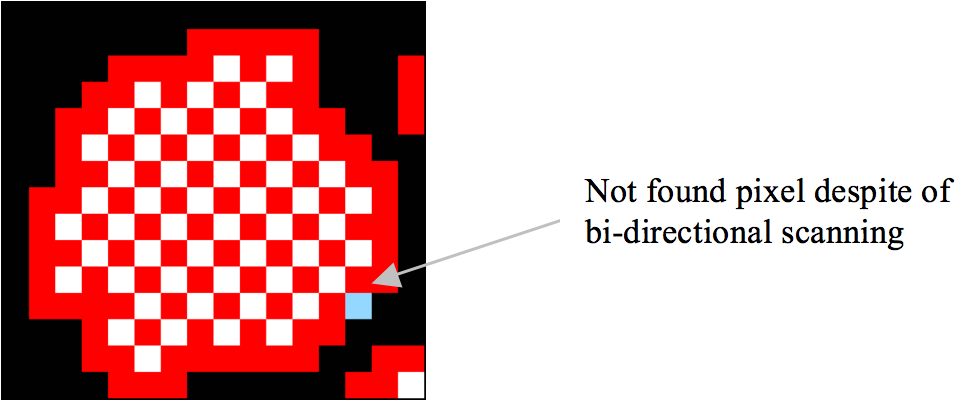
\includegraphics[width=0.6\textwidth]{5.ExperimentalResult/fig22.png}
	\caption{Result of the proposed algorithm by using bidirectional scanning.}
	\label{fig:image22}
\end{figure}

\JHMEMO{See comment!}
%\JHMEMO{21 b와 c 가 차이가 없어 보임, 22에서 지적한 점이 c에서 찾아져야 할 것 같음}

In the experiments, there were some missing contour pixels that did not satisfy the experimental conditions described in \cite{Danielsson1981Improvement}. In figures \ref{fig:img21-b} and \ref{fig:img21-c}, there are eight untraced contour pixels because the horizontal scan line cannot find a starting pixel for the contour under some conditions. In other words, since the scan line seeks an untraced black pixel with an adjacent white pixel on the horizontal line, if the untraced contour pixel which is between two black pixels in the horizontal direction has an adjacent white pixel in the vertical and/or diagonal direction, the untraced contour pixel cannot be considered as the starting pixel. Therefore, as shown in \textcolor{red}{Table 7}, the missing contour pixels remain after running the proposed algorithm and the untraced contour pixels of other algorithms are also included in the missing contour pixels due to the same problem. In particular, image \#9 has the largest number of missing contour pixels because it has many one-pixel-sized chessboard patterns that comprise inner-outer corner pixels. The chessboard pattern consists of one-pixel-sized inner-outer corner pixels, which tend to cause the missing start pixel problem. 

To overcome the problem, we can apply an 8 connection mask to the images for obtaining the starting pixel, but the mask requires many operations. In other words, we made an attempt to measure the performance of multidirection scanning for eliminating the missing contour pixels problem by using vertical and horizontal scans instead of 8 connection mask operation. \textcolor{red}{Table 12} shows the increase in the number of pixels traced by using bidirectional scanning, and \textcolor{red}{Table 13} describes the processing time for this method. Moreover, figure \ref{fig:image22} shows the tracing result obtained by using the proposed algorithm based on bidirectional scanning, and it shows that seven of the missing pixels are traced but still one diagonal connective contour pixel \textcolor{red}{(A)} is untraced. 

In the above tables, bidirectional scanning slightly increases the number of traced contour pixels, but their processing time increases dramatically. Moreover, the proposed algorithm shows acceptable performance in terms of accuracy $(99.5\%)$, although only unidirectional scanning is performed. Hence, unidirectional scanning based on the proposed algorithm is sufficient for application to contour tracing under the condition that a relatively small number of objects are present and real-time tracing such as AR, MR, and recognition-image-based code is performed on small-scale images such as those in a mobile computing environment.